\subsection{Algemeen concept}
Voor de testen werdt gebruik gemaakt van een simpele server waar clients op kunnen verbinden. De client kan vervolgens het absolute tijd verschil meten met een atomische wereld klok. 

Eerst en vooral is er een vertraging tussen een aangesloten client en de server, de {\it ping}. Dit is gemeten in miliseconden.
Deze wordt gemeten door een bericht met de actuele tijd te verzenden van de server naar de client, en terug. De verzonden tijd wordt afgetrokken van de actuele tijd waarmee de ping verkregen is.
In figuur \ref{diag} is de informatieoverdracht zichtbaar. In de server wordt de servertijd (TS1) berekent door middel van een worldtime API die de exacte wereld tijd teruggeeft, verzonden naar de client en teruggekregen. 
Nu wordt de actuele tijd berekent in de server TS2. Dus de uiteindelijke ping is:
\[ping = TS2 - TS1\]

\begin{figure}
\centering
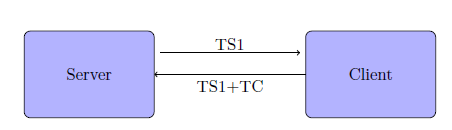
\includegraphics[scale=0.8]{img/img.png}
\caption{Ping} \label{diag}
\end{figure}


Het is niet gegarandeerd dat de klokken van de clients allemaal gesynchroniseerd zijn met de server.
Bij het terug verzenden van de client naar de server wordt de clienttijd (TC) bij het bericht gezet. Met deze TC en de berekende {\it ping}, is het mogelijk het tijdsverschil tussen de client en de server te bepalen ($DeltaTime$).
\[DeltaTime = (TC+ping/2) - TS2\]
Dit is de data die zal worden bekenken en vergeleken tussen browsers en besturings systemen.

\subsection{UDP vs TCP}

UDP heeft in tegenstelling tot TCP geen verbinding nodig tussen bijvoorbeel server en client. TCP zal garanderen dat data correct aankomt door middel van error checking en zal ook in de goede volgorde binnen stromen. Zodat geen packeten worden verloren zal TCP deze in een receive buffer steken en zal de applicatie de data pas lezen als ze er klaar voor is. Dit in tegenstelling tot UDP waar de data continue zal binnen stromen, ontvangen of niet. Hier wordt ook geen error checking uitgevoerd en de volgorde is niet gegarandeerd. Het is duidelijk dat UDP veel sneller is doordat er veel minder moet worden gedaan. Dit is ook de reden dat het NTP protocol UDP zal gebruiken in plaats van TCP. Het is logisch dat voor een simpele synchronisatie tussen client en server geen complex protocol nodig is.
Socket.io gebruikt het TCP protocol. 



\subsection{Analyse van de data}